Tout d'abord, il faut définir $P_{dBm}$. Le schéma du microphone qui nous est donné permet de réaliser les calculs.

\begin{figure}[htb]
    \centering
    \includegraphics[width=0.8\textwidth]{schemabloc_méthode1.png}
    \caption{Schéma bloc microphone}
    \label{fig:Schéma_Fonctionnel_1}
\end{figure}

En effet, nous avons la relation suivante :
\begin{equation}
P_{dBm} = 10 \times \log(V_a^2 \times 1000) \ \text{avec}\ V_a = S \times P_a
\end{equation}
Cependant, S la sensibilité \footnote{\href{http://electroacoustique.univ-lemans.fr/cours/Grain1.2/co/grain2_2_2.html}{Pour la formule de la sensibilité S}} que l'on nous donne est en dBV et pas en $V/P_a$, il faut donc la convertir. Nous savons que :\begin{equation}
    S = 20\times \log(\frac{S_{v/Pa}}{S_{ref}}) \ \text{avec}\  S_{ref} = 1 V/P_a
\end{equation} donc :
\begin{equation}
   S_{V/P_a} = S_{ref}*10^\frac{S}{20} 
\end{equation}
Nous avons donc :
\begin{equation}
V_m = S_{V/P_a} \times P_a
\end{equation} 
Pour $P_a$, nous utilisons la formule de $P_{SPL}$ \footnote{\href{https://fr.wikipedia.org/wiki/Pression_acoustique}{Pour la formule de $P_{SPL}$}}: 
\begin{equation}
    P_{SPL} = 20\times \log(\frac{P_a}{P_{ref}}) 
\end{equation}
d'où :
\begin{equation}
P_a = P_{ref} * 10^{\frac{P_{SPL}}{20}}
\end{equation}
Il ne reste que le gain à traiter, celui-ci s'exprime en dB dans les paramètres donnés, or, nous voulons l'exprimer sans unité, nous obtenons alors 
\begin{equation}
    G_{SU} = 10^\frac{G}{20} \ \text{où} \ G_{SU} \ \text{est sans unité} \footnote{\href{https://fr.wikipedia.org/wiki/Gain_d\%C3\%A9cibel}{Pour la formule du gain sans unité $G_{SU}$}}
\end{equation}

Cela nous permet de trouver la formule finale : 
\\
\tcbox[colback=yellow!20, colframe=yellow, boxrule=2pt]{$ P_{dBm} = 10 \times \log((G_{SU} \times S_{VPA} \times P_a)^2 \times 1000)$}
En substituant avec les résultats précédents, on obtient :
\tcbox[colback=green!20, colframe=green, boxrule=2pt]{$P_{dBm} = 20 \times \log(10^\frac{G}{20} \times S_{REF} \times 10^{\frac{S}{20}} \times P_{REF} \times 10^{\frac{P_{SPL}}{20}})+30$}
Enfin, avec : \begin{itemize}
    \item $S_{REF} = 1$
    \item $P_{REF} = 20 \mu Pa$
    \item $G = 40 dB$
    \item $S = -48 dBV$
    \item $P_{SPL} = 80 dB SPL$
\end{itemize} 
On obtient : \tcbox[colback=green!20, colframe=green, boxrule=2pt]{$P_{dBm} = 8 dBm$.}
À présent, nous avons la valeur de $P_{dBm}$ qui va nous servir de référence. Pour chaque signal, nous allons le décomposer en plusieurs « sous-signaux » à chaque fois que la valeur de référence est franchie. 
Par exemple, sur la figure \ref{Fig.1.2}, on distingue trois « sous-signaux » ou plages de signal différentes, car la valeur de référence est franchie deux fois. Ensuite, chaque plage est traitée comme un nouveau signal et, si cette plage se trouve au-dessus de la valeur référence et dure plus d’une seconde, alors le son de cette plage est catalogué dans la catégorie bruit pénible. Sur cet exemple, il y a donc deux sons acceptables (plages 1,3) et un son pénible (plage 2).
Enfin, pour chaque signal, on règle la taille des fenêtres d’analyse pour obtenir un résultat correct, contenant 2k+1 échantillons.Pour déterminer la puissance instantanée, nous utilisons la formule suivante :
\begin{equation}
    P(n) = \frac{1}{2K+1}\sum_{n-K}^{n+K}_{x(k)^2}
\end{equation}
L'identification du paramètre k ainsi que le choix de sa valeur retenue dépendent de la nature du signal et des exigences spécifiques de l'analyse. Admettons que nous avons un signal de 5s et d'une fréquence de 20k Hz, si k = 80, on aura 161 échantillons par fenêtre. Pour un signal sonore, il faut que la taille de la fenêtre soit petite, car c'est un fichier son. Pour avoir un bon vecteur puissance à analyser, il faut donc une fenêtre inférieure à la seconde, comme on a Te, il faut déterminer k tel que :
\begin{equation}
    k < \frac{(\frac{1}{Te}-1)}{2}
\end{equation}
\begin{figure}[htb]
    \centering
    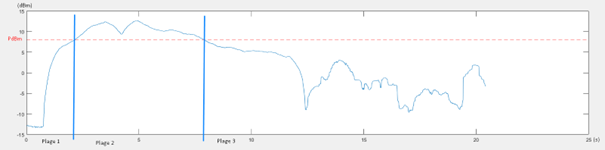
\includegraphics[width=0.8\textwidth]{Exemple_seuil_se_pénibilité.png}
    \caption{Exemple signal avec plages acceptables et pénibles}
    \label{Fig.1.2}
\end{figure}

